\documentclass{article}
\usepackage{mathtools}
\usepackage{mathrsfs}
\usepackage{graphicx}
\graphicspath{ {./images/} }

\mathtoolsset{showonlyrefs}  
\begin{document}
\title{Pendulum Cart System}
\author{Grant Fitez}
\maketitle
\section{Introduction}
\paragraph{Goal} The pendulum cart system is intended to demonstrate the motion of a system derived using Lagrangian mechanics. This system was chosen as it meets all of the following criteria:
\begin{itemize}
	\item The system should have the potential to be chaotic: A tiny change in the initial conditions should result in a much larger and relatively unpredictable change as the system evolves.
	\item It should not be possible to easily derive the equations of motion using Newtonian mechanics.
	\item  It should be possible to easily create a visual representation of the system over time.
	\item The system should theoretically conserve energy, allowing for a way to check the accuracy of the simulation. 
\end{itemize}
\paragraph{Description of system} Let f(x) be an arbitrary continuous, twice differentiable function on a 2 dimensional plane. Along f(x) there is a "cart" or a point of mass M which is allowed to travel freely along the path f(x). Attached to the "cart" is another point of mass m, which is attached to the original mass by a weightless rod of length $\ell$. The secondary mass and rod are allowed to rotate freely around the first mass, essentially creating a pendulum. The two variable coordinates in this system are the x position of the first mass (x) and the angle between the two masses measured from the -y axis ($\theta$).
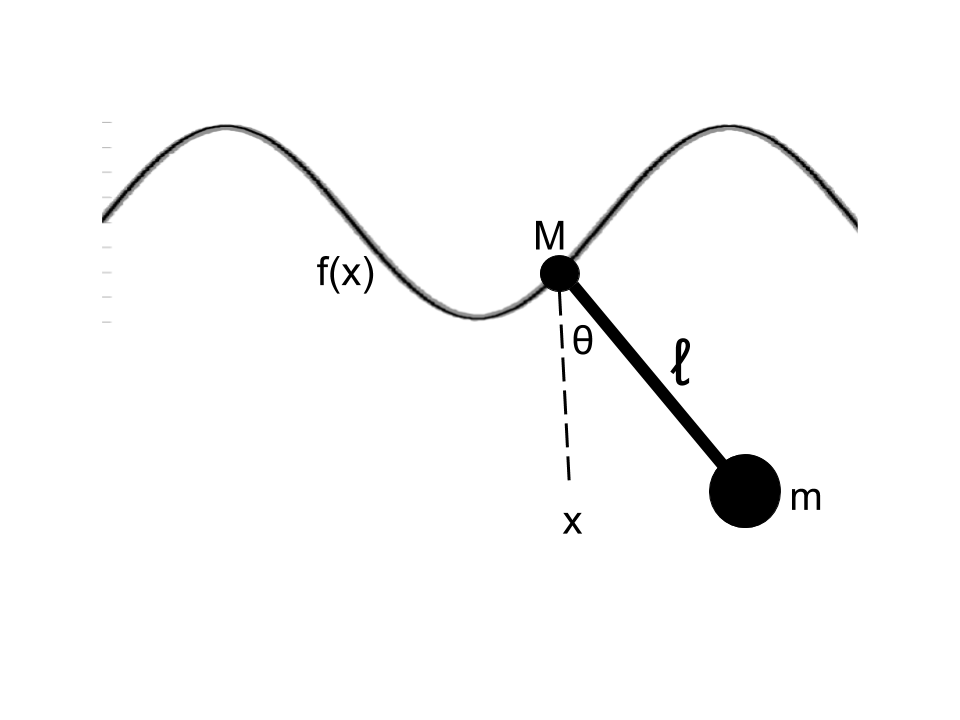
\includegraphics[width=\textwidth,height=\textheight,keepaspectratio]{Pendulum_Cart.png}
\section{Finding the Lagrangian}

\subsection{Definitions of Points}
\begin{gather}
M_x=x \\
M_y=f(x)\\
m_x=x+\ell sin(\theta)\\
m_y=f(x)-\ell \cos(\theta)
\end{gather}
\\
\subsection{Derivatives of Points}
\begin{gather}
\dot{M_x}=\dot x \\
\dot{M_y}=f'(x)\dot x \\
\dot{m_x}=\dot x+\ell \cos(\theta)\dot{\theta} \\
\dot{m_y}=f'(x)\dot x +\ell sin(\theta)\dot{\theta}
\end{gather}
\subsection{Kinetic Energy of System}
\[
T=\frac M2 (\dot x ^2 + (f'(x)\dot x)^2) + \frac m2 ((\dot x+\ell \cos(\theta)\dot{\theta})^2+(f'(x)\dot x +\ell sin(\theta)\dot{\theta})^2)
\]
\[
T=\frac M2 (\dot x ^2 + f'(x)^2\dot x^2)+\frac m2 (\dot x ^2 +2\dot x \ell \cos(\theta)\dot{\theta}+\ell^2cos^2(\theta)\dot\theta^2 + f'(x)^2\dot x ^2 +2f'(x)\dot x \ell sin(\theta) \dot\theta + \ell^2 sin^2(\theta)\dot \theta^2)
\]
\[
T=\frac M2 \dot x ^2(1 + f'(x)^2)+\frac m2 (\dot x ^2 +2\dot x \ell \cos(\theta)\dot{\theta} + f'(x)^2\dot x ^2 +2f'(x)\dot x \ell sin(\theta) \dot\theta + \ell^2 \dot \theta^2)
\]
\[
T=\frac M2 \dot x^2(1+f'(x)^2)+\frac m2 \dot x^2[1+f'(x)^2]+\frac m2(2\dot x \dot \theta \ell[\cos(\theta)+f'(x)sin(\theta)]+\ell^2\dot \theta^2)
\]
\[
T=\frac{M+m}2 \dot x^2(1+f'(x)^2)+m \dot x \dot \theta \ell (\cos(\theta)+f'(x)sin(\theta))+\frac m2 \ell^2
\dot \theta^2
\]
\subsection{Potential Energy of System}
\[V=Mgf(x)+mg(f(x)-\ell \cos(\theta))\]
\[V=Mgf(x)+mgf(x)-mg\ell \cos(\theta) \]
\subsection{Lagrangian}
\[\mathscr{L}=T-V\]
\[
\mathscr{L}=\frac{M+m}2 \dot x^2(1+f'(x)^2)+m \dot x \dot \theta \ell (\cos(\theta)+f'(x)\\sin(\theta))+\frac m2 \ell^2
\dot \theta^2-Mgf(x)-mgf(x)+mg\ell \cos(\theta)
\]


\section{Solving the Euler-Lagrange Equation}
\subsection{Solving Equation for x}
\subsubsection{Solving for $\frac{\partial\mathscr L}{\partial \dot x}$}
\[
\frac{\partial \mathscr L}{\partial \dot x}
=(M+m)\dot x (1+f'(x)^2)+m \ell(\dot \theta \cos(\theta)+\dot \theta f'(x)\sin(\theta))
\]
\[
\frac{\partial \mathscr L}{\partial \dot x}
=(M+m)\dot x + (M+m)\dot x f'(x)^2 +m\ell\dot \theta\cos\theta+m\ell\dot\theta f'(x)\sin\theta
\]
\subsubsection{Solving for $\frac{d}{dt}\frac{\partial\mathscr L}{\partial \dot x}$}
\begin{equation}
\begin{aligned}
\frac d{dt}\frac{\partial \mathscr L}{\partial \dot x}=
(M+m)\ddot x+[(M+m)\ddot xf'(x)^2+2(M+m)\dot xf'(x)f''(x)\dot x]+[ml\ddot \theta \cos\theta-m\ell\dot\theta^2\sin\theta]
\\+[m\ell\ddot \theta f'(x)\sin\theta+m\ell\dot\theta f''(x)\dot x \sin\theta +m\ell\dot\theta f'(x)\cos\theta\dot\theta]
\end{aligned}
\end{equation}
\subsubsection{Solving for $\frac{\partial\mathscr L}{\partial x}$}
\[
\frac{\partial \mathscr L}{\partial x}
=(M+m)\dot x^2f'(x)f''(x)+m\dot x\ell \dot \theta \sin \theta f''(x)-Mgf'(x)-mgf'(x)
\]

\subsubsection{Final equation}
\begin{equation}
\begin{aligned}
(M+m)\ddot x+(M+m)\ddot xf'(x)^2 +2(M+m)\dot x^2f'(x)f''(x)+m\ell\ddot\theta\cos\theta-m\ell\dot\theta^2\sin\theta\\+m\ell\ddot\theta f'(x)\sin\theta+m\ell\dot\theta^2f'(x)\cos\theta=(M+m)\dot x^2 f'(x)f''(x)-Mgf'(x)-mgf'(x)
\end{aligned}
\end{equation}
\subsection{Solving for $\theta$}
\subsubsection{Solving for $\frac{\partial\mathscr L}{\partial \dot \theta}$}
\[
\frac{\partial\mathscr{L}}{\partial\dot\theta}
=m \ell( \dot x \cos(\theta)+ \dot x f'(x)\sin(\theta))+m \ell^2 \dot \theta
\]
\subsubsection{Solving for $\frac{d}{dt}\frac{\partial\mathscr L}{\partial \dot x}$}
\[
\frac {d}{dt} \frac{\partial\mathscr{L}}{\partial\dot\theta}=
[m\ell\ddot x\cos\theta-m\ell\dot x\sin\theta\dot\theta]+[m\ell\ddot x f'(x)\sin\theta+m\ell\dot x^2 f''(x)\sin\theta+m\ell\dot xf'(x)\cos\theta\dot\theta]+m\ell^2\ddot\theta
\]
\subsubsection{Solving for $\frac{\partial\mathscr L}{\partial \theta}$}
\[\frac{\partial\mathscr{L}}{\partial\theta}=
-m\dot x\ell\dot\theta\sin\theta+m\dot x \ell \dot\theta f'(x)\cos\theta-mg\ell\sin\theta
\]
\subsubsection{Final equation}
\begin{equation}
\begin{aligned}
m\ell\ddot x\cos\theta-m\ell\dot x\sin\theta\dot\theta+m\ell\ddot xf'(x)\sin\theta+m\ell\dot x^2 f''(x)\sin\theta+m\ell\dot x f'(x)\cos\theta\dot\theta+m\ell^2\ddot\theta\\=-m\dot x\ell\dot\theta\sin\theta+m\dot x\ell\dot\theta f'(x)\cos\theta-mg\ell\sin\theta
\end{aligned}
\end{equation}
\\
\[
m\ell\ddot x\cos\theta+m\ell\ddot x f'(x)\sin\theta+m\ell\dot x^2 f''(x)\sin\theta+m\ell^2\ddot\theta=-mg\ell\sin\theta
\]
\section{Finding the Equations of Motion}
The equations of motion can be derived from the two equations from the previous sections: 
\[
m\ell\ddot x\cos\theta+m\ell\ddot x f'(x)\sin\theta+m\ell\dot x^2 f''(x)\sin\theta+m\ell^2\ddot\theta=-mg\ell\sin\theta
\]
and
\begin{equation}
\begin{aligned}
(M+m)\ddot x+(M+m)\ddot xf'(x)^2 +2(M+m)\dot x^2f'(x)f''(x)+m\ell\ddot\theta\cos\theta-m\ell\dot\theta^2\sin\theta\\+m\ell\ddot\theta f'(x)\sin\theta+m\ell\dot\theta^2f'(x)\cos\theta=(M+m)\dot x^2 f'(x)f''(x)-Mgf'(x)-mgf'(x)
\end{aligned}
\end{equation}
\subsection{Isolating $\ddot x$ and $\ddot \theta$}
\begin{equation}
\begin{aligned}
\ddot x=[-2(M+m)\dot x^2f'(x)f''(x)-m\ell\ddot\theta\cos\theta+m\ell\dot\theta^2\sin\theta-m\ell\ddot\theta f'(x)\sin\theta-m\ell\dot\theta^2f'(x)\cos\theta\\+(M+m)\dot x^2 f'(x)f''(x)-Mgf'(x)-mgf'(x)]/(M+m)(1+f'(x)^2)
\end{aligned}
\end{equation}

\begin{equation}
\begin{aligned}
\ddot \theta=\frac{-g\sin\theta-\ddot x\cos\theta-\ddot xf'(x)\sin\theta-\dot x^2f''(x)\sin\theta}{\ell}
\end{aligned}
\end{equation}
\subsection{Substitute $\ddot x$ and $\ddot \theta$ Into Each Other and Solve}
\begin{equation}
\begin{aligned}
\ddot x=[-2(M+m)\dot x^2f'(x)f''(x)+mg\sin\theta\cos\theta+m\dot x^2 f''(x)\sin\theta\cos\theta+m\ell\dot\theta^2\sin\theta+mgf'(x)\sin^2\theta\\+m\dot x^2 f'(x)f''(x)\sin^2\theta-m\ell\dot\theta^2f'(x)\cos\theta+(M+m)\dot x^2f'(x)f''(x)-Mgf'(x)-mgf'(x)]\\/[(M+m)(1+f'(x)^2)-m\cos^2\theta-mf'(x)\sin\theta\cos\theta-mf'(x)\cos\theta\sin\theta-mf'(x)^2\sin^2\theta]
\end{aligned}
\end{equation}

\begin{equation}
\begin{aligned}
\ddot \theta=[-g\sin\theta-\frac{\cos\theta+f'(x)\sin\theta}{(M+m)(1+f'(x)^2)}[-2(M+m)\dot x^2f'(x)f''(x)+m\ell\dot\theta^2\sin\theta\\-m\ell\dot\theta^2f'(x)\cos\theta+(M+m)\dot x^2f'(x)f''(x)-mgf'(x)-Mgf'(x)]-\dot x^2f''(x)\sin\theta]\\/[\ell-\frac{m\ell}{(M+m)(1+f'(x)^2)}(\cos^2\theta+f'(x)\sin\theta\cos\theta+f'(x)\sin\theta\cos\theta+f'(x)^2\sin^2\theta)]
\end{aligned}
\end{equation}










\end{document}